\setcounter{figure}{0}

\section{8th October 2023: I AM the bread of life}
\subsection*{Text: John 6:35-58}
  \begin{quote}
    [35] Jesus said to them, “I am the bread of life; whoever comes to me shall not hunger, and whoever believes in me shall never thirst. [36] But I said to you that you have seen me and yet do not believe. [37] All that the Father gives me will come to me, and whoever comes to me I will never cast out. [38] For I have come down from heaven, not to do my own will but the will of him who sent me. [39] And this is the will of him who sent me, that I should lose nothing of all that he has given me, but raise it up on the last day. [40] For this is the will of my Father, that everyone who looks on the Son and believes in him should have eternal life, and I will raise him up on the last day.”

    [41] So the Jews grumbled about him, because he said, “I am the bread that came down from heaven.” [42] They said, “Is not this Jesus, the son of Joseph, whose father and mother we know? How does he now say, ‘I have come down from heaven’?” [43] Jesus answered them, “Do not grumble among yourselves. [44] No one can come to me unless the Father who sent me draws him. And I will raise him up on the last day. [45] It is written in the Prophets, ‘And they will all be taught by God.’ Everyone who has heard and learned from the Father comes to me—[46] not that anyone has seen the Father except he who is from God; he has seen the Father. [47] Truly, truly, I say to you, whoever believes has eternal life. [48] I am the bread of life. [49] Your fathers ate the manna in the wilderness, and they died. [50] This is the bread that comes down from heaven, so that one may eat of it and not die. [51] I am the living bread that came down from heaven. If anyone eats of this bread, he will live forever. And the bread that I will give for the life of the world is my flesh.”

    [52] The Jews then disputed among themselves, saying, “How can this man give us his flesh to eat?” [53] So Jesus said to them, “Truly, truly, I say to you, unless you eat the flesh of the Son of Man and drink his blood, you have no life in you. [54] Whoever feeds on my flesh and drinks my blood has eternal life, and I will raise him up on the last day. [55] For my flesh is true food, and my blood is true drink. [56] Whoever feeds on my flesh and drinks my blood abides in me, and I in him. [57] As the living Father sent me, and I live because of the Father, so whoever feeds on me, he also will live because of me. [58] This is the bread that came down from heaven, not like the bread the fathers ate, and died. Whoever feeds on this bread will live forever.”
  \end{quote}
\subsection*{Notes}
\begin{itemize}
  \item{Jesus is the bread of life -> not just one food option amongst many. Eating or not eating this bread is a matter of life and death, it is a matter of eternal satisfaction. }
  \item{But why can we trust in Jesus claim that those who eat this bread will live forever?}
  \item{Three points today: Jesus’ identity, Jesus’ mission, and whether Jesus was successful in His mission}
  \item{Jesus’ identity: prior to this bread of life discourse was the feeding of the 5000. For the Jews, this was a throwback to God’s promise that one day, God will raise up a prophet like Moses. So the Jews thought that just like how Moses gave bread everyday, this Jesus can also give food everyday.
  \begin{itemize}
    \item{in light of this misunderstanding of the Jews, Jesus said: “I AM the bread of life”. Jesus saying that he is greater than Moses. First of all, it was not even Moses who gave the bread, it was God. But secondly, Jesus himself is the bread that gives eternal life. Jesus is the \textbf{provider} as well as the \textbf{provision}. In the past, God provided for Israel in quite impersonal ways. But now, we have “whoever comes to ME”, “whosoever believes in ME, everyone who looks to the Son”, etc. The Son of God has come into the world himself to provide for the world in a more personal way. }
  \end{itemize}}
  \item{Also, while God sent manna to sustain lives temporarily, God sent Jesus to transform our lives spiritually and to give us eternal life. And even in the OT, the manna had a special significance (c.f Deuteronomy 8:3). Even in the OT, the manna was not about solely meeting the physical needs of the Israelites, but the was about meeting the spiritual needs of the Israelites. And in the NT, what was alluded to in the OT finds its fulfilment. }
  \item{Jesus has come to do the Father’s will, which is to save us. Jesus has come to provide himself as the spiritual sustenance that leads to eternal life. The manna that God provided in the past hinted at God’s spiritual provision for his people, and that as the OT people trusted in God’s word, they would live. But now, when the Son of God himself comes in the flesh, when we trust in the Som of God, we would live forever.}
  \item{And Jesus says that “whoever comes to me shall not hunger, whoever believes in me shall never thirst”. There is on-going satisfaction in Jesus when we believe in Him. All our spiritual needs are met, are satisfied, when we believe in Jesus. This is truly the fulfilment of what is promised in Deut 8:3. And this meeting of our spiritual needs would lead to godly contentment even when our physical needs aren’t met. }
  \item{The problem with human nature is not desire. Without desire, we would be robots. The problem with human nature is either desiring the wrong things, or desiring neutral things inordinately. Part of the solution to that is that when we desire God as the highest good for us, and when we desire all neutral things insofar as it is rooted on a desire for God, then that is part of the solution to our sin. The other part of the solution is Jesus’ promise here, that all who come to Him and eat His flesh will never hunger. All who desire Him and believe in Him will be satisfied. }
  \item{Some people rejected Jesus’ message. First reason was that they thought that his birth was too common for the big claims that he was making. }
  \item{Second reason was “How can this man give us his flesh to eat?” The listeners interpreted Jesus’ statement literally, and they rejected Jesus on that basis. }
  \item{But ultimately, the reason for the listeners rejection was because of God’s sovereign will. People can only come to Jesus unless it is granted him by the Father. God’s sovereign and gracious drawing is both necessary and sufficient, and that is our hope as we share the gospel. }
  % \item{\begin{figure}[H] \centering
  %   % 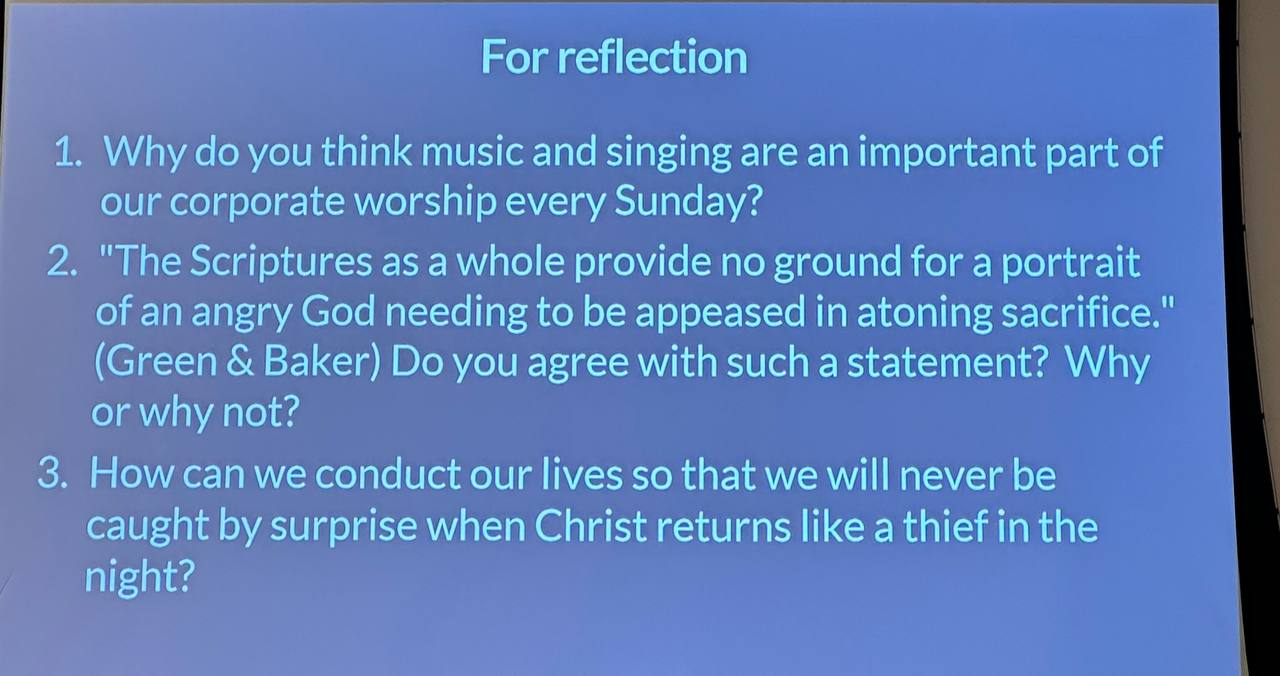
\includegraphics[width=0.8\textwidth, trim={0cm 0cm 0cm 0cm},clip]{Figures/marchSermon4Reflections.jpg}
  %   \includegraphics[width=0.8\textwidth, trim={0cm 0cm 0cm 0cm},clip]{example-image-a}
  %   \caption[]{Reflection questions for this sermon}
  %   \label{}
  % \end{figure}}
\end{itemize}